\chapter{研究過程}
寫出你的研究過程與相關資料收集的內容.....

\blindtext[1]


\chapter{研究結果展示}
%\section{研究分析}
資料分析方法
本研究利用統計分析套件軟體 SPSS 20進行相關分析,使用的分析如下
\begin{enumerate}
\item 描述性統計 :分析樣本結構中性別,年紀教育,程度工作性質的百分比
\item 信度分析:以Cronbach's 值來鑑定各量表的內部一致性
\item 因素分析:主要目的將原有很多變數(維度)之資料,縮減成較少的維度數,但有保持原本所提供的資料
\item 簡單迴歸:分析進行假設的驗證
\end{enumerate}

本研究探討品牌知覺、品牌聲望、消費者滿意度之間的關係。本研究已發放問卷的方式取的資料,問卷填寫主要以網路發放題目主要
品牌知覺、品牌聲望、消費者滿意度以簡單迴歸分析來驗證假設是否成立

變數的定義與衡量
\begin{enumerate}
\item 品牌知覺共有8個題目商品的品質良好、鈦鍺品牌形象	、製作材料(與特性)、商品外觀設計很滿意、商品的廣告或名稱很滿意、整體商品的價值、品牌知名度
\item 品牌聲望共有10個題目價錢、品牌形象、製作材料(與特性)、其他顧客反應、商品認證保證、售後服務、交貨服務、整體商品的價值、品牌知名度、設計感
\item 消費者滿意度共有10題目價錢、品牌形象、製作材料(與特性)、其他顧客反應、商品認證保證、售後服務、交貨服務、整體商品的價值、品牌知名度、設計感
\end{enumerate}
分析結果
本研究採用網路與百貨公司附近發放方式,針對可能聽過鈦鍺精品的人進行問卷調查供調查603份剔除重複填寫與漏填,有效問卷599份 
本研究的樣本資料分析結果顯示 
\begin{enumerate}
\item 男性佔 50.1 % 女性 49.3% 如表 \ref{tab:PL1} 所示 
\item 年齡分為18歲以下 9.6% 、19 ~25歲 71.5% 、26~35歲 9.8%、36~40歲2.7% 、40歲以上5.8%本問卷族群與年輕族群居多。如表  \ref{tab:PL2} 所示
\item 教育方面 高中以下4.1%、高中(職)19.4%、專科5.3%、大學64.1%、碩士5.3%、博士1.7% 教育程度以大學64.1%為最多 。如表 \ref{tab:PL3} 所示
\item 工作性質 學生52.4%、服務業29.4%、製造業3.5%、軍公教4.3%、自由業8.5%、管家1.3%由職業可看以學生64.1%為最高。如表 \ref{tab:PL4} 所示
\end{enumerate}

\begin{table}[htb]
\caption{基本資料 (性別)}
\label{tab:PL1}
\renewcommand{\arraystretch}{1.2} % 將表格行間距加大為原來的 1.2 倍
\arrayrulewidth=1pt               % 調整線條粗細為 1pt
\tabcolsep=24pt                   % 調整欄間距為 24pt
%\begin{document}
\begin{tabular}[t]{lll}  % 第一欄位使用 sans serif 字族
\hline
 & $次數$ & $百分比$ \\
\hline
男生        & 302 & 50.1 \\
女生        & 297  & 49.3 \\
總和        & 599  & 99.3 \\
遺漏值            & 4 & 0.7 \\
\hline
\centering
\label{fig:PL4}
\end{tabular}
\end{table}

\begin{table}[htb]
\caption{基本資料 (年齡)}
\label{tab:PL2}
\renewcommand{\arraystretch}{1.2} % 將表格行間距加大為原來的 1.2 倍
\arrayrulewidth=1pt               % 調整線條粗細為 1pt
\tabcolsep=18pt                   % 調整欄間距為 24pt
%\begin{document}
\begin{tabular}[t]{lll}  % 第一欄位使用 sans serif 字族
\hline
 & $次數$ & $百分比$ \\
\hline
18歲以下        & 58  & 9.6 \\
19~25歲        & 431  & 71.5 \\
26~35歲        & 59  & 9.8 \\
36~40歲        & 16  &2.7\\
40歲以上        & 35  & 5.8 \\
總和               & 599  & 99.3 \\
遺漏值            & 4 & 0.7 \\
\hline
\end{tabular}
\end{table}

\begin{table}[htb]
\caption{基本資料 (學歷)}
\label{tab:PL3}
\renewcommand{\arraystretch}{1.2} % 將表格行間距加大為原來的 1.2 倍
\arrayrulewidth=1pt               % 調整線條粗細為 1pt
\tabcolsep=18pt                   % 調整欄間距為 24pt
%\begin{document}
\begin{tabular}[t]{lll}  % 第一欄位使用 sans serif 字族
\hline
 & $次數$ & $百分比$ \\
\hline
高職以下       & 25  & 4.1 \\
高中(職)        & 116  & 19.2 \\
專科        & 32  & 5.3 \\
大學        & 384 &63.7\\
碩士        & 32  & 5.3 \\
博士           & 10  & 1.7 \\
總和           & 599  & 99.3 \\
遺漏值            & 4 & 0.7 \\
\hline
\end{tabular}
\end{table}

\begin{table}[htb]
\caption{基本資料 (工作性質)}
\label{tab:PL4}
\renewcommand{\arraystretch}{1.2} % 將表格行間距加大為原來的 1.2 倍
\arrayrulewidth=1pt               % 調整線條粗細為 1pt
\tabcolsep=18pt                   % 調整欄間距為 24pt
\begin{tabular}[t]{lll}  % 第一欄位使用 sans serif 字族
\hline
 & $次數$ & $百分比$ \\
\hline
學生           & 316  & 52.4 \\
服務業        & 177  & 29.4 \\
製造業        & 21  & 3.5 \\
軍公教        & 26  &4.3\\
自由業        & 51  & 8.5 \\
家管           & 8  & 13 \\
總和               & 599  & 99.3 \\
遺漏值            & 4 & 0.7 \\
\hline
\end{tabular}
\end{table}

首先對樣本收集已說明,其次對本研究的變數衡量做信度分析最後驗證假設
信度分析:已進行實證分析針對問卷問項進行信度分析用來得知問卷設計所測得的結果是否有信度與穩定性本研究採用目前已研究最常使用的 信賴度數做信度量測指標 Nunnally(1978)認為信度0.7以上表示高信度 可接受值大於0.7

本研究共有 3個變數,信度分析結果顯示
\begin{enumerate}
\item 品牌知覺Cronbach's Alpha 值 0.936  如表 \ref{tab:e1}  所示
\item 品牌聲望Cronbach's Alpha 值  0.958 如表 \ref{tab:e2}  所示
\item 消費者滿意度Cronbach's Alpha 值 0.969 如表 \ref{tab:e3}  所示
\end{enumerate}
以上信度 Alpha 值 大於 0.7以上顯示本研究的變數具有不錯的可信度。


\begin{table}[htb]
\caption{信度 (品牌知覺)}
\label{tab:e1}
\renewcommand{\arraystretch}{1.2} % 將表格行間距加大為原來的 1.2 倍
\arrayrulewidth=1pt               % 調整線條粗細為 1pt
\tabcolsep=6pt                   % 調整欄間距為 24pt
\begin{tabular}[t]{lllll}  % 第一欄位使用 sans serif 字族
\hline
 & $代號$& $平均數$ & $標準差$& $ Alpha 值 $ \\
\hline
品牌知覺 & 知覺1  & 3.7753   & 0.7479  &0.936242 \\
              & 知覺2  & 3.7483  &0.79497  &  \\
             & 知覺3  & 3.8345    & 0.80373  &  \\
             & 知覺4 & 3.7500   &0.75513  &\\
             & 知覺5   & 3.7534  & 0.77393 &  \\
             & 知覺6  & 3.7534    &  0.77393 & \\
             & 知覺7  & 3.6909     & 0.80231  &  \\
\hline
\end{tabular}
\end{table}

\begin{table}[htb]
\caption{信度 (品牌聲望)}
\label{tab:e2}
\renewcommand{\arraystretch}{1.2} % 將表格行間距加大為原來的 1.2 倍
\arrayrulewidth=1pt               % 調整線條粗細為 1pt
\tabcolsep=6pt                   % 調整欄間距為 24pt
\begin{tabular}[t]{lllll}  % 第一欄位使用 sans serif 字族
\hline
 & $代號$& $平均數$ & $標準差$& $ Alpha 值 $ \\
\hline
品牌知覺 & 聲望1  & 3.6835 &0.82500 &0.958532\\
              & 聲望2  & 3.7089 &0.83439 &  \\
             & 聲望3  &3.5949 &0.85266  &  \\
             & 聲望4  &3.6456&0.75987\\
             & 聲望5  & 3.7468 &0.83924 &  \\
             & 聲望6  & 3.6456&0.78508& \\
             & 聲望7  & 3.6709&0.77900  &  \\
             & 聲望8  & 3.7215&0.84636&  \\
             & 聲望9  &3.6456&0.81709&  \\
             & 聲望10  & 3.7848&0.82696 &  \\
\hline
\end{tabular}
\end{table}

\begin{table}[htb]
\caption{信度 (消費者滿意度)}
\label{tab:e3}
\renewcommand{\arraystretch}{1.2} % 將表格行間距加大為原來的 1.2 倍
\arrayrulewidth=1pt               % 調整線條粗細為 1pt
\tabcolsep=6pt                   % 調整欄間距為 24pt
\begin{tabular}[t]{lllll}  % 第一欄位使用 sans serif 字族
\hline
 & $代號$& $平均數$ & $標準差$& $ Alpha 值 $ \\
\hline
品牌知覺 & 滿意度1&3.233&0.97143&0.969024\\
              & 滿意度2&3.4667&1.10589&  \\
             & 滿意度3&3.5000&1.00858&  \\
             & 滿意度4&3.5667&1.13512&\\
             & 滿意度5&3.7000&1.08755&  \\
             & 滿意度6&3.5667&1.16511&\\
             & 滿意度7&3.4667&1.00801&  \\
             & 滿意度8&3.6333&0.99943&  \\
             & 滿意度9&3.4333&1.04000&\\
             & 滿意度10&3.5667&1.07265&\\
\hline
\end{tabular}
\end{table}

因素分析
為了探討受訪者對主要考量因素,因此提出8題品牌知覺、10題品牌知覺、10題消費者滿意度等變數以量表收集受訪者對每一變數之重視度(非常不同意=1、非常同意=5)。將所獲得之資料,經過KMO取樣適當性及巴氏球形檢定。
\begin{enumerate}
\item 品牌知覺
KMO=0.926 大於0.9表示分析效果極佳 Bartlett 的球形檢值 3210.519 顯著性.000<α = 0.01 顯示資料非常適合因素分析  本部分特性值大於1之標準將7個變數濃縮為1個因變數(主成分)全部變異之72.457可解釋為72.457%,詳細的數據如表  \ref{tab:p4} 所示。
\item 品牌聲望
KMO=0.899 大於0.8表示分析有價值 Bartlett 的球形檢值 800.032 顯著性.000<α= 0.01 顯示資料非常適合因素分析  本部分特性值大於1之標準將7個變數濃縮為1個因變數(主成分)全部變異之73.020可解釋為73.020% 如圖 \ref{tab:p4}  所示。
\item 消費者滿意度
KMO=0.788 大於0.7表示分析中等 Bartlett 的球形檢值 420.646 顯著性.000<0.01 顯示資料非常適合因素分析  本部分特性值大於1之標準將7個變數濃縮為1個因變數(主成分)全部變異之78.632可解釋為78.632% 如圖 \ref{tab:p4} 所示
\end{enumerate}

\begin{table}[htb]
\caption{因數分析}
\label{tab:p4}
\renewcommand{\arraystretch}{1.2} % 將表格行間距加大為原來的 1.2 倍
\arrayrulewidth=1pt               % 調整線條粗細為 1pt
\tabcolsep=6pt                   % 調整欄間距為 24pt
\begin{tabular}[t]{llll}  % 第一欄位使用 sans serif 字族
\hline
 $因素分析$& $KMO$ & $Bartlett$& $全部異變數$ \\
\hline
 滿意度1&3.233&0.97143&0.969024\\
 滿意度2&3.4667&1.10589&  \\
 滿意度3&3.5000&1.00858&  \\
\hline
\end{tabular}
\end{table}

%\begin{figure}[!t]
%\centering
%\includegraphics[width=8cm]{images/kom.PNG}
%\caption{因素分析}
%\label{fig:p4}
%\end{figure}

假設之驗證
本研究共有3個假設待驗證,均採用簡單迴歸分析,結果整理於表 \ref{fig:p7} 所示以下對每個假設驗證結果加以說明
\begin{enumerate}
\item H1.品牌知覺與品牌聲望有顯著的關係。
以簡單迴歸分析得值為:簡單相關數0.480 判定數(R平方)為0.231調過的R平方數為0.220,滿意度與聲望迴歸值為0.492其t值4.678 顯著性值為=0.000<α=0.05,結果為棄卻因變數與自變數間無迴歸關係存在之虛無假設;自變數與因變數間有存在直線關係,因此可看出品牌知覺與品牌聲望有顯著的關係之假設=成立。如表 \ref{tab:r1}  所示。
\item H2.品牌知覺與消費者滿意度有顯著的關係。
以簡單迴歸分析得值為意度與知覺為0.060其t值0.647 顯著性值為=0.524<α=0.05結果為無法棄卻因變數與自變數間無迴關關係純在之虛無假設;自變數與因變數間無存在直線關係因此可看出品牌聲望與消費者滿意度有顯著的關係之假設=不成立。如表 \ref{tab:r3}  所示。
\item H3.品牌聲望與消費者滿意度有顯著的關係。
以簡單迴歸分析得值為:簡單相關數為0.893 判定數(R平方)為0.798調過的R平方數為0.780,滿意度與聲望迴歸值為0.692其t值7.832 顯著性值為=0.000<α=0.05, 結果為棄卻因變數與自變數間無迴歸關係存在之虛無假設;自變數與因變數間有存在直線關係,因此可看出品牌知覺與消費者滿意度有顯著的關係之假設=成立。如表 \ref{tab:r2}  所示。

\end{enumerate}



\begin{figure}[!t]
\centering
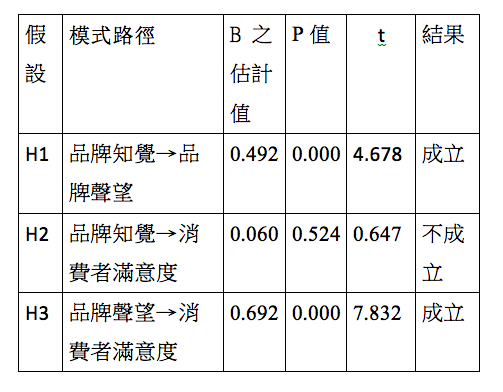
\includegraphics[width=8cm]{images/H.PNG}
\caption{假設}
\label{fig:p7}
\end{figure}

\begin{table}[htb]
\caption{簡單回歸(依變數:知覺的構面)}
\label{tab:r1}
\renewcommand{\arraystretch}{1.2} % 將表格行間距加大為原來的 1.2 倍
\arrayrulewidth=1pt               % 調整線條粗細為 1pt
\tabcolsep=6pt                   % 調整欄間距為 24pt
\begin{tabular}[t]{llllll}  % 第一欄位使用 sans serif 字族
\hline
 $模型$&$B估計值$&$標準誤差$& $Beta分配$& $t$& $顯著性$ \\
\hline
(常數)&0.249&0.105&0.480&2.375&0.020\\
聲望的構面&0.492&0.105&0.480&4.678&0.00\\
\hline
\end{tabular}
\end{table}

\begin{table}[htb]
\caption{簡單回歸(依變數:滿意度構面)}
\label{tab:r2}
\renewcommand{\arraystretch}{1.2} % 將表格行間距加大為原來的 1.2 倍
\arrayrulewidth=1pt               % 調整線條粗細為 1pt
\tabcolsep=6pt                   % 調整欄間距為 24pt
\begin{tabular}[t]{llllll}  % 第一欄位使用 sans serif 字族
\hline
 $模型$&$B估計值$&$標準誤差$& $Beta分配$& $t$& $顯著性$ \\
\hline
(常數)&0.158&0.103&&1.531&0.140\\
聲望的構面&0.692&0.088&0.857&7.832&0.000\\
\hline
\end{tabular}
\end{table}

\begin{table}[htb]
\caption{簡單回歸(依變數:滿意度構面)}
\label{tab:r3}
\renewcommand{\arraystretch}{1.2} % 將表格行間距加大為原來的 1.2 倍
\arrayrulewidth=1pt               % 調整線條粗細為 1pt
\tabcolsep=6pt                   % 調整欄間距為 24pt
\begin{tabular}[t]{llllll}  % 第一欄位使用 sans serif 字族
\hline
 $模型$&$B估計值$&$標準誤差$& $Beta分配$& $t$& $顯著性$ \\
\hline
(常數)&0.158&0.103&&1.531&0.140\\
知覺的構面&0.060&0.093&0.071&0.647&0.524\\
\hline
\centering
\end{tabular}
\end{table}


\chapter{結論與建議}

結論請分成下列幾點依序說明。

\section{結論}
\blindtext[1]


\section{未來發展建議}

\blindtext[1]

\section{後續研究方向}

\blindtext[1]

\chapter{研究生必讀:如何交代你的「研究方法」}

在論文中如何交代你的「研究方法」?

在論文中,「研究方法」一節必須回答以下兩個問題:一是資料是如何搜集到或者衍生出來的,二是資料是如何分析的。換句話說,你要告訴讀者你是怎樣得到你的研究結果的。

但是為甚麼你須要解釋你怎樣得到你的研究結果呢?不習慣現代西洋人學術思考方式的華人研究者,對此也許會感到困惑不解。他們在撰寫研究計劃或者論文本文時經常不曉得要寫些甚麼,尤其不曉得為甚麼要花那麼大的力氣去交代研究過程,好像過程比結果更重要 ──結果不對而過程對可以是好論文,反而結果對而過程不對就不是好論文,沒有瞎貓抓到死老鼠這種好事。以下姑且依據西洋人對學術論文的可能想法,列出六點理由略加說明。這六點理由同時亦間接指示了我們應該往甚麼方向去交代我們的研究方法:

\begin{enumerate}[1., noitemsep]
\item 因為研究方法會影響到研究結果。譬如說,如果你在探討台北市捷運乘客對台北市捷運效能的看法,而你所使用的是可作多項選擇的問卷而不是對個別乘客進行訪談,那麼你所得到的結果就會有所不同。讀者若知道你用甚麼方法得到資料,即有助於他評估你的研究結果是否有效和可信。

\item 同一個研究問題可以有多種探究方法,你必須交代為何你決定選用某種方法來研究,而捨棄別的相關方法。
\item 讀者也想知道你得到資料的方式是否合於探究主題之常理。譬如說,如果你使用問卷調查法來探究台北市捷運乘客對於捷運效能的看法,而你的問卷中卻只提供「1.非常好2.很好3.好」等三種正向選擇的回答而完全不提供負向選擇的回答,即不合於此種探究主題之常理。
\item 讀者也想判斷你所使用的研究方法是否協合於研究目標。譬如在上述所例舉的探究中,你只個案研究一位乘客,這顯然就不協合於研究目標。
\item 你也必須談一下你如何預防本來預期會發生的問題,而假如真有問題發生時你又如何把問題的衝擊力道減到最低。
\item 如果你交代得夠清楚的話,有時候別的研究者會直接採用或者變相借用你的研究方法論(研究方法交代方式),特別是你的研究方法論頗有新意,又或者借用者慧眼獨具之時。
\end{enumerate}


至於在全篇論文中又該在甚麼地方和以甚麼方式交代你的研究方法呢?當然最重要的是「研究方法」這一章節了。在這一章節中你必須集中而扼要地說明你的研究方法。不過,並不是在這一章節中交代過就算了事了。在論文的其他章節中,也須適時酌量附帶說明一下。以下依論文章節安排略為提點一下:

\begin{itemize}[noitemsep]
\item 【緒論】研究問題介紹、研究目標介紹、研究程序介紹、主要研究結果與結論之選擇性介紹
\item 【文獻回顧】回顧與你的研究問題有關的已有文獻(針對它們如何界定、說明和正當化此一研究問題而談)、回顧已有的相關研究方法論文獻(同樣針對它們如何界定、說明和正當化而談)、回顧已有的相關研究結果文獻(特別針對可信度等來談)
\item 【研究方法】對獲取資料的方式和分析資料的方式詳加解釋、對方法論問題及其解決辦法和效果加以說明
\item 【研究結果及討論】研究結果之呈現、關於研究結果之詮釋與延伸討論(譬如跟已有的研究結果作比較等)
\item 【結論】說明研究問題是否有所「解答」、在何種程度上本研究達成了目標、我們從此研究結果中學到甚麼、從此研究結果中所學到的知識有甚麼用、此研究有何缺點等等
\end{itemize}

一般初學的研究者在交代研究方法時常犯有以下幾種錯誤:
\begin{enumerate}[1., noitemsep]
\item 無關的細節講太多。
\item 不必要的初學者方法知識和程序細節仍然交代得清清楚楚,徒增篇幅。
\item 忽略了討論搜集資料時所遇到的問題,以及沒有交代如何克服困難和權衡輕重時的考量點。
\end{enumerate}

以下介紹一些比較常見的研究類型:

\begin{enumerate}[1., noitemsep]

\item 【個案研究】(case study)對於一個或多個個人、團體、社群、企業或機構之背景、現況、環境和發展歷程予以觀察、記錄、分析,就其內部和外部的諸種影響而言得出某些階段性的變化模式來。
\item 【比較研究】(comparative study)比較兩個或多個情況之間的異同。
【相關與預測的研究】(correlation-prediction study)求得一些因素之間在統計上有顯著意義的相關係數,並且加以詮釋,以作為預測未來類同情況之參考。
\item 【評估研究】(evaluation study)判斷某種計劃或安排是否遵循預定的程序並且達成其明說的目標。
\item 【設計與展示的研究】(design-demonstration study)建構、測試和評估新的體系或新的程式是否可行。
\item 【實驗研究】(experimental study)對控制其中一項或多項變異因素所求得的結果加以分析。
\item 【問卷調查研究】(survey-questionnaire study)以問卷方式對某個特定團體的行為、信念和意見予以確定、報導並詮釋。
\item 【狀態特性研究】(status study)對於一個或多個現象之代表性案例或者取樣案例加以觀察檢驗,以確定其特殊性格。
\item 【理論建構研究】(theory construction study)尋找或描述一些可解釋事物之所以如此運作的原理。
\item 【趨勢分析研究】(trend analysis study)分析目前事件之動力結構以便預測或預斷事件之未來走向。
\item 【概念分析研究】(concept analysis study)對於某些學術上使用的關鍵性概念作語意方面或邏輯方面的分析。
\end{enumerate}
